In diesem Abschnitt sollen verschiedene Ma{\ss}nahmen gegen Cyber Sickness vorgestellt werden. Dar\"uberhinaus soll erkl\"art werden, warum diese wirkungsvoll sind und was m\"ogliche Nachteile bei der Nutzung entsprechder Ma{\ss}nahmen sein k\"onnten.

Die Ma{\ss}nahmen lassen sich in auf Grund der Sensory Conflict Theory in drei Kategorien einteilen:
Reduktion der Inkongruenz der visuellen Reize entgegen der Erfahrung, indem diese optimiert werden (\autoref{Visuals}), Generation von kongruenten, vestibul\"aren Stimuli entsprechend der Erwartung durch die visuellen Reize (\autoref{Vestibular}) und Adaptation durch den Organismus selbst (\autoref{Adaptation}). Eine generell zu erkennende Tendenz besteht darin, dass diese Methoden versuchen, eine gewohnte \textbf{Nat\"urlichkeit} in der virtuellen Umgebung zu erzeugen.

\subsection{Anpassung der visuellen Reize}\label{Visuals}
Eine Vection passiert dann, wenn ein \textbf{statischer Referenzpunkt} fehlt, an dem man sich optisch fixieren und somit seine Lage relativ dazu sicher feststellen kann. Dies passiert beispielsweise, wenn man aus einem Zug auf einen anderen schaut, ohne den Himmel sehen zu k\"onnen. Wenn der andere Zug sich in Bewegung setzt, erlebt man kurzzeitig Vection, da hier der Himmel als statische Referenz fehlte.

Daher kann ein unabh\"angiger Hintergrund, vorrangig bei CAVE Displays, nach Duh et al.\cite{Duh:2001:Static} helfen. Nat\"urlich ist die Methoden beispielsweise bei Head-Mounted Displays nicht nutzbar, da diese die visuelle Wahrnehmung der tats\"achlichen Umgebung vollst\"andig ersetzen. Eine Methode dennoch einen bekannten Fixpunkt in die virtuelle Umgebung zu integrieren ist die virtuelle Nase wie in \autoref{abb:vnose}, die laut Wienrich et al.\cite{Wienrich:2018:Nose} die Intensit\"at von Cyber Sickness bei Nutzung von Head-Mounted-Displays reduzieren kann.


\begin{figure}[b]
	\centering 
	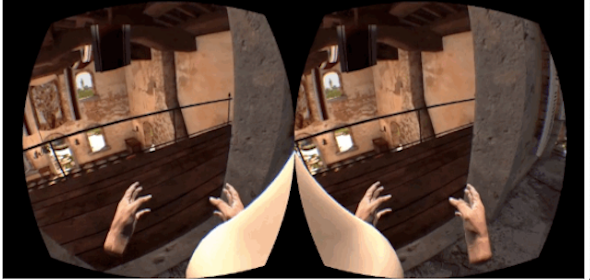
\includegraphics[width=\columnwidth]{virtual_nose.png}
	\caption{Virtuelle Nase zur Reduktion von Cyber Sickness bei Head-Mounted Displays. Bild von WIRED\cite{WIRED:2020:Nose}, letzter Zugriff: 03.05.2020}
	\label{abb:vnose}
\end{figure}


Desweiteren ist es f\"ur die Reduktion von Cyber Sickness ratsam, wenn die graphische Darstellung und Design der virtuellen Umgebung sich dadurch auszeichnen, dass sie nat\"urlich wirken und ruhige, weite Szenen ohne schnellwechselnde Bewegungen nachbildet. Die Parameter der Graphik sollten wie folgt umgesetzt werden:

Die Aufl\"osung und Wiederholungsrate\footnote{50-60 Hz, nach Simon et al.\cite{Simon:2014:Factors}} sollten angemessen hoch sein\cite{kirollos:2019:refresh}, das \textit{Field of View} sollte sich nach Fernandes et al.\cite{Fenandes:2016:FOV} dynamisch anpassen und tendenziell eher klein sein und hoch \"uber dem Boden ansetzen, sofern der Kontext, für den die virtuelle Umgebung genutzt wird, das zulässt. Geringe Latenz f\"uhrte nach Meehan et al.\cite{Meehan:2003:latency} zu mehr wahrgenommener Presence und laut Simon et al.\cite{Simon:2014:Factors} auch zu Cyber Sickness, ebenso wie durch Flickern in der Darstellung der virtuellen Umgebung.
Bei all diesen Punkten stellt sich immer die Frage des Aufwandes und der Umsetzbarkeit durch die verfügbare Hardware.

Es scheint, als verursachen realistischere Graphik bzw. Animationen stärkere Cyber Sickness\cite{Pouke:2018:Realism}.
In Anbetracht der beiden Punkte, statische Referenz und Natürlichkeit, empfehlen sich weite Landschaften in virtuellen Umgebungen und im Sinne der Sensory Conflict Theory, Fortbewegung in Virtual Reality m\"oglichst zu reduzieren\footnote{In Computerspielen zum Beispiel Teleportation nutzen}, wobei sich hier erneut das Problem aufwirft, dass diese Methoden nicht in jedem Kontext der Virtual Reality einsetzbar sind.

Obwohl mit den genannten Anpassung der visuellen Komponente die Vection schon wesentlich angenehmer und weniger gestört durch Cyber Sickness sein kann, sodass auch eine Immersion in die virtuelle Umgebung stattfindet, ist es immer möglich zusätzlich kongruente, vestibuläre Stimuli zu erzeugen, sodass die Vection keine Illusion mehr ist, sondern nahe an das tatsächliche Bewegungserlebnis herankommt.


\subsection{Erzeugen kongruenter Stimuli}\label{Vestibular}



\subsection{Adaption an die Inkongruenz}\label{Adaptation}
Age simon et al.
Gender 
Illness
Posture
andere Sinne

Control
Duration